\documentclass[a4paper,12pt]{article}
\usepackage{xcolor}
\usepackage{amsmath,amsfonts,amssymb}
\usepackage{geometry}
\usepackage{fancyhdr}
\usepackage{graphicx}
\usepackage{titlesec}
\usepackage{tikz}
\usepackage{booktabs}
\usepackage{array}
\usetikzlibrary{shadows}
\usepackage{tcolorbox}
\usepackage{float}
\usepackage{lipsum}
\usepackage{mdframed}
\usepackage{pagecolor}
\usepackage{mathpazo}   % Palatino font (serif)
\usepackage{microtype}  % Better typography

% Page background color
\pagecolor{gray!10!white}

% Geometry settings
\geometry{margin=0.5in}
\pagestyle{fancy}
\fancyhf{}

% Fancy header and footer
\fancyhead[C]{\textbf{\color{blue!80}CS754 Assignment-1}}
% \fancyhead[R]{\color{blue!80}Saksham Rathi}
\fancyfoot[C]{\thepage}

% Custom Section Color and Format with Sans-serif font
\titleformat{\section}
{\sffamily\color{purple!90!black}\normalfont\Large\bfseries}
{\thesection}{1em}{}

% Custom subsection format
\titleformat{\subsection}
{\sffamily\color{cyan!80!black}\normalfont\large\bfseries}
{\thesubsection}{1em}{}

% Stylish Title with TikZ (Enhanced with gradient)
\newcommand{\cooltitle}[1]{%
  \begin{tikzpicture}
    \node[fill=blue!20,rounded corners=10pt,inner sep=12pt, drop shadow, top color=blue!50, bottom color=blue!30] (box)
    {\Huge \bfseries \color{black} #1};
  \end{tikzpicture}
}
\usepackage{float} % Add this package

\newenvironment{solution}[2][]{%
    \begin{mdframed}[linecolor=blue!70!black, linewidth=2pt, roundcorner=10pt, backgroundcolor=yellow!10!white, skipabove=12pt, skipbelow=12pt]%
        \textbf{\large #2}
        \par\noindent\rule{\textwidth}{0.4pt}
}{
    \end{mdframed}
}

% Document title
\title{\cooltitle{CS754 Assignment-3}}
\author{{\bf Saksham Rathi, Ekansh Ravi Shankar, Kshitij Vaidya}}
\date{}

\begin{document}
\maketitle
\textbf{Declaration:} The work submitted is our own, and
we have adhered to the principles of academic honesty while completing and submitting this work. We have not referred to any unauthorized sources, and we have not used generative AI tools for the work submitted here.

\section*{Question 2}

\begin{solution}{Solution}

  \section{Linear System Representation}
  The coded snapshot equation \( E = \sum_{t=1}^T \mathbf{C}_t \odot \mathbf{F}_t \) can be rewritten as the linear system:
  \[
  \mathbf{A} \mathbf{x} = \mathbf{b},
  \]
  where:
  \begin{enumerate}
      \item \(\mathbf{x}\) is the **vectorized unknown video sequence**, formed by stacking the vectorized frames \(\mathbf{F}_t\):
      \[
      \mathbf{x} = \begin{bmatrix}
      \text{vec}(\mathbf{F}_1) \\
      \text{vec}(\mathbf{F}_2) \\
      \vdots \\
      \text{vec}(\mathbf{F}_T)
      \end{bmatrix} \in \mathbb{R}^{HWT \times 1}.
      \]
      
      \item \(\mathbf{b}\) is the **vectorized coded snapshot**:
      \[
      \mathbf{b} = \text{vec}(E) \in \mathbb{R}^{HW \times 1}.
      \]
      
      \item \(\mathbf{A}\) is the **measurement matrix** encoding the modulation by \(\mathbf{C}_t\). It is a block-diagonal matrix with horizontally concatenated diagonal matrices:
      \[
      \mathbf{A} = \begin{bmatrix}
      \text{diag}(\text{vec}(\mathbf{C}_1)) & \text{diag}(\text{vec}(\mathbf{C}_2)) & \cdots & \text{diag}(\text{vec}(\mathbf{C}_T))
      \end{bmatrix} \in \mathbb{R}^{HW \times HWT}.
      \]
      Each block \(\text{diag}(\text{vec}(\mathbf{C}_t))\) is a diagonal matrix whose entries are the vectorized binary code \(\mathbf{C}_t\) for frame \(t\).
  \end{enumerate}

\end{solution}

\begin{figure}[htbp]
    \centering
    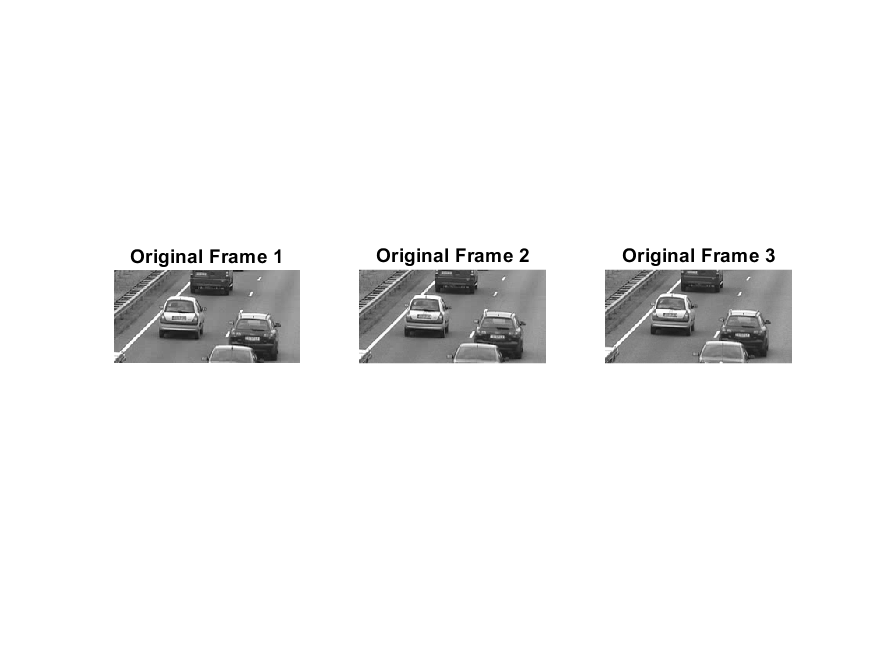
\includegraphics[width=0.8\textwidth]{../images/original_frames.png}
    \caption{Original Frames for T = 3}

\end{figure}

\begin{figure}[htbp]
    \centering
    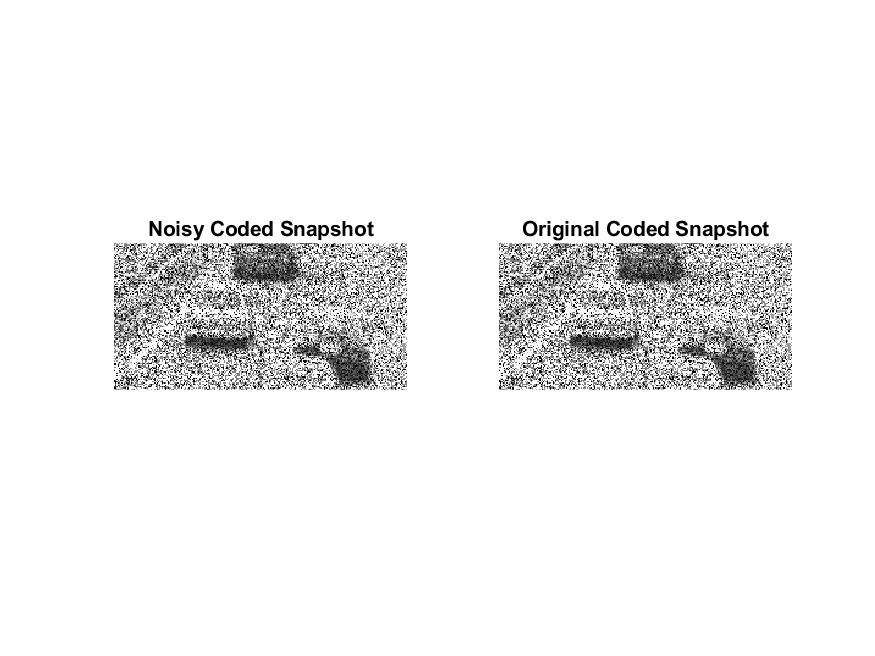
\includegraphics[width=0.8\textwidth]{../images/noisy_coded_snapshot.png}
    \caption{Encoded Snapshot for T = 3}

\end{figure}

\begin{figure}[htbp]
    \centering
    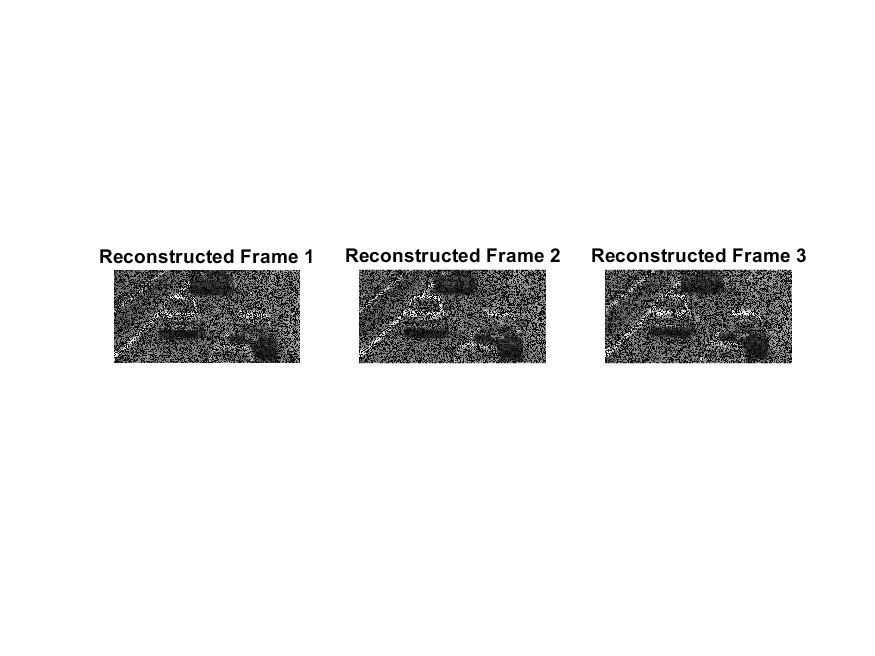
\includegraphics[width=0.8\textwidth]{../images/reconstructed_frames.png}
    \caption{Reconstructed Frames for T = 3}

\end{figure}

\begin{figure}[htbp]
  \centering
  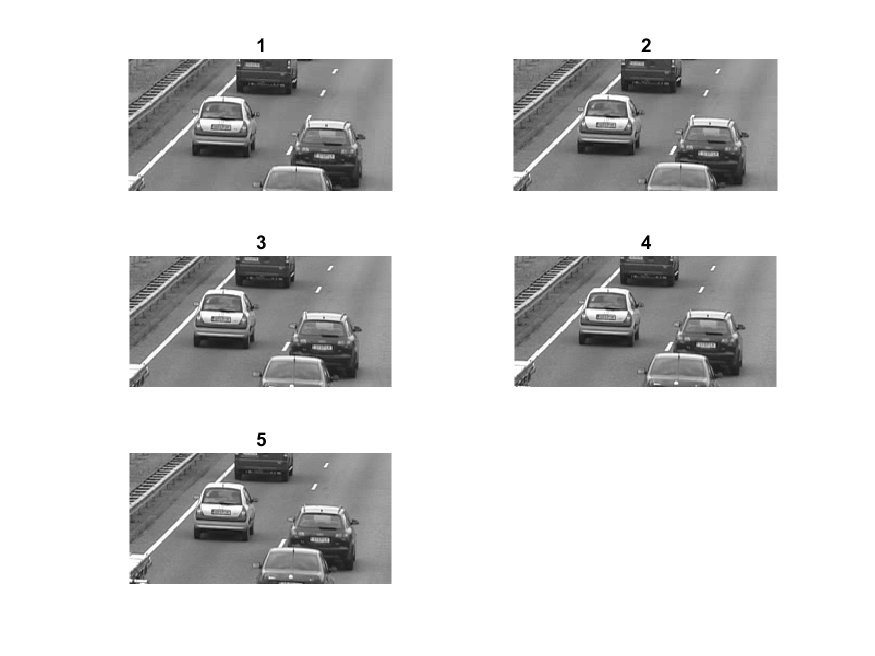
\includegraphics[width=0.8\textwidth]{../images/original_frames_5.png}
  \caption{Original Frames for T = 5}
\end{figure}

\begin{figure}[htbp]
  \centering
  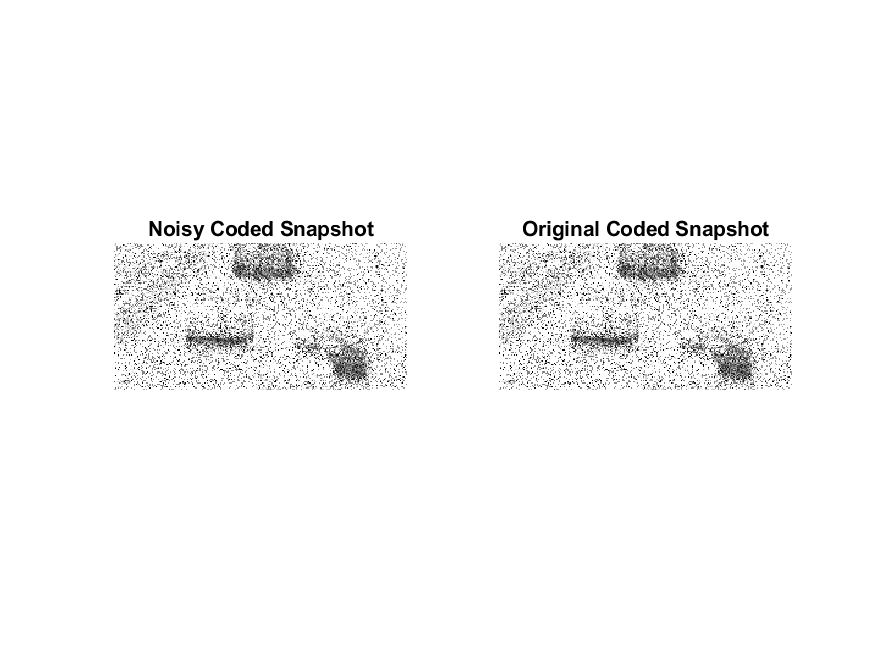
\includegraphics[width=0.8\textwidth]{../images/noisy_coded_snapshot_5.png}
  \caption{Encoded Snapshot for T = 5}
\end{figure}

\begin{figure}[htbp]
  \centering
  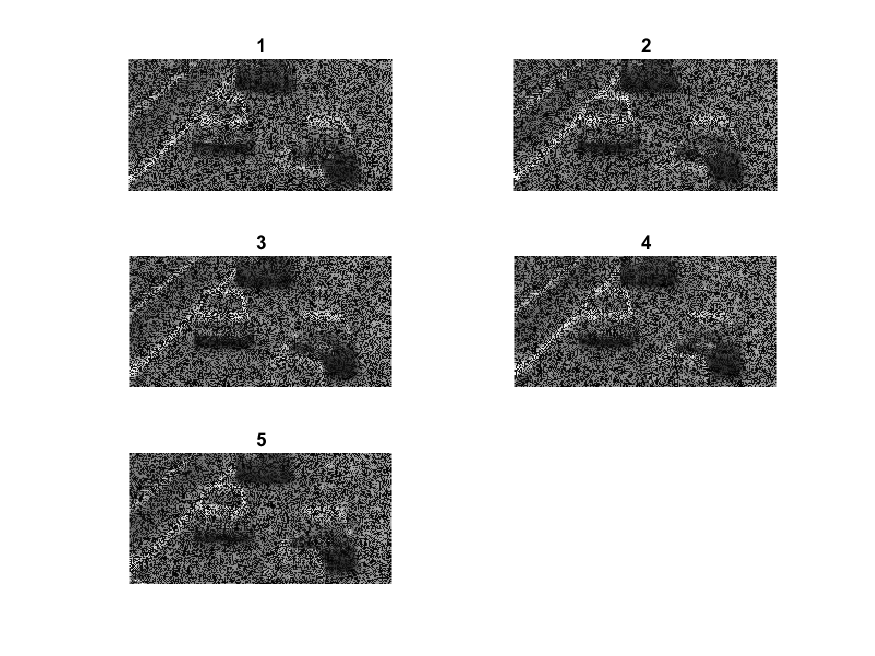
\includegraphics[width=0.8\textwidth]{../images/reconstructed_frames_5.png}
  \caption{Reconstructed Frames for T = 5}
\end{figure}

\begin{figure}[htbp]
  \centering
  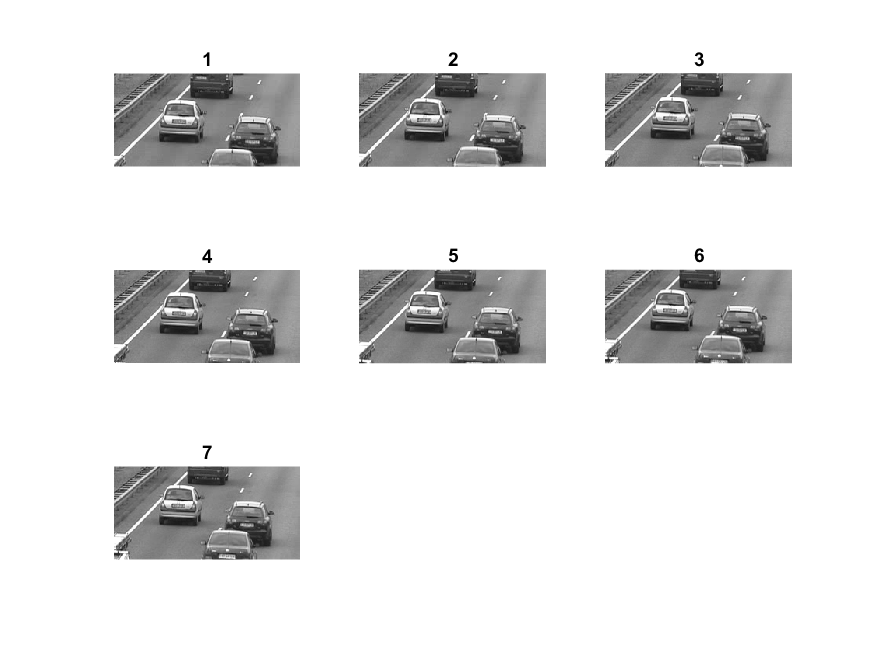
\includegraphics[width=0.8\textwidth]{../images/original_frames_7.png}
  \caption{Original Frames for T = 7}
\end{figure}

\begin{figure}[htbp]
  \centering
  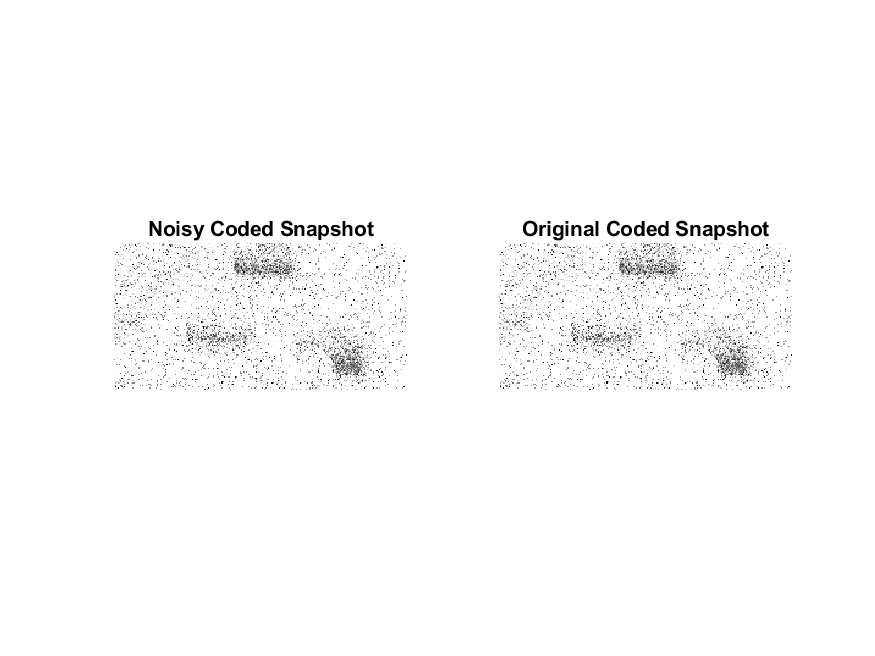
\includegraphics[width=0.8\textwidth]{../images/noisy_coded_snapshot_7.png}
  \caption{Encoded Snapshot for T = 7}
\end{figure}

\begin{figure}[htbp]
  \centering
  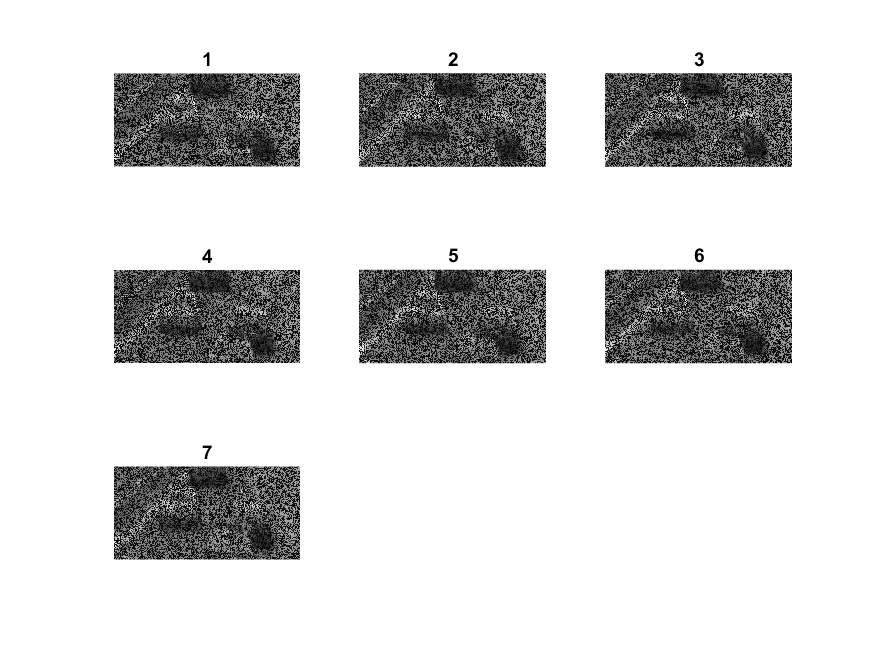
\includegraphics[width=0.8\textwidth]{../images/reconstructed_frames_7.png}
  \caption{Reconstructed Frames for T = 7}
\end{figure}

\begin{figure}[htbp]
  \centering
  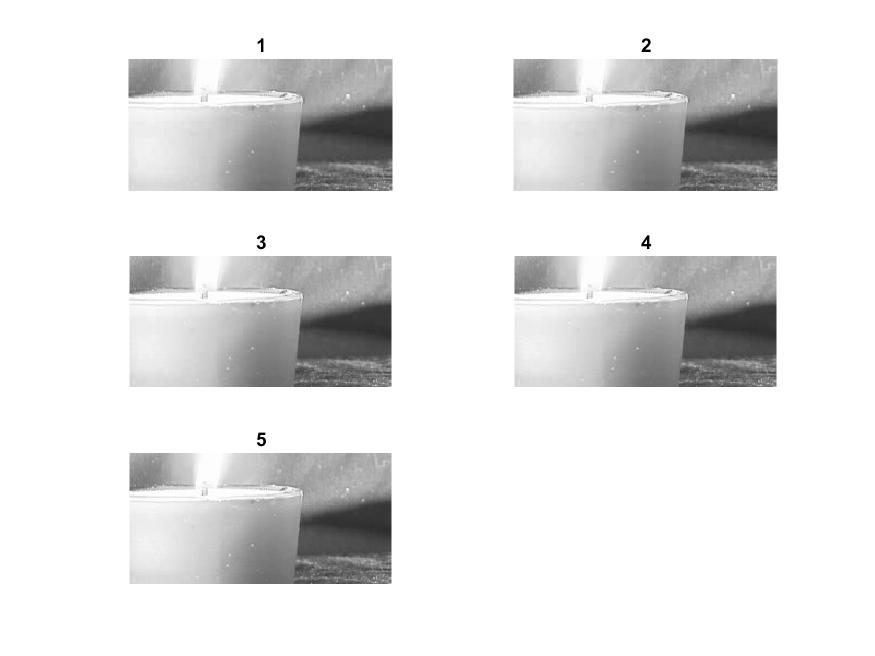
\includegraphics[width=0.8\textwidth]{../images/original_frames_flame.png}
  \caption{Original Frames for T = 5 : Flame Video}
  \label{fig:output}
\end{figure}

\begin{figure}[htbp]
  \centering
  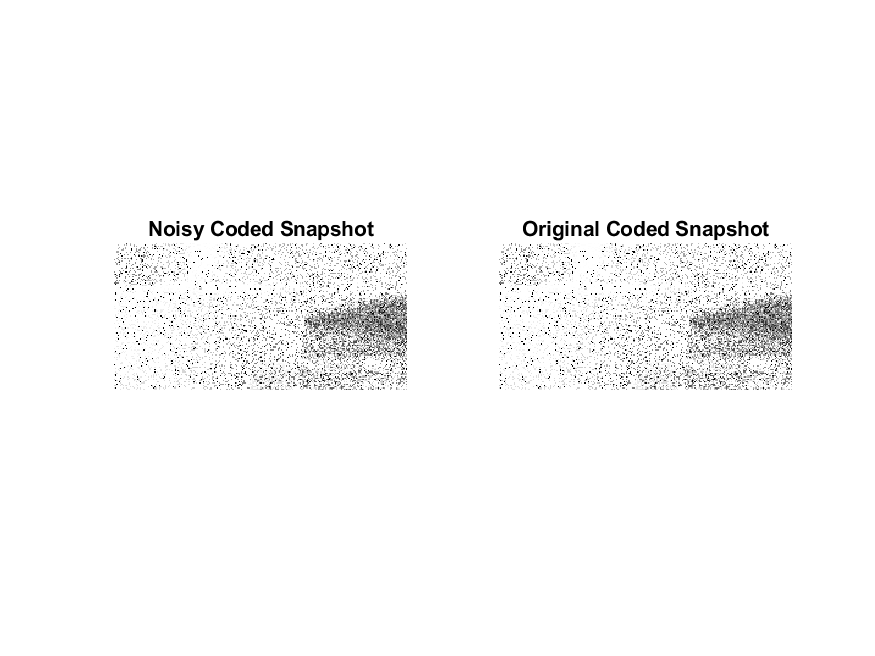
\includegraphics[width=0.8\textwidth]{../images/noisy_coded_snapshot_flame.png}
  \caption{Encoded Snapshot for T = 5 : Flame Video}
  \label{fig:output}
\end{figure}

\begin{figure}[htbp]
  \centering
  \includegraphics[width=0.8\textwidth]{../images/reconstructed_frames_flame.png}
  \caption{Reconstructed Frames for T = 5 : Flame Video}
  \label{fig:output}
\end{figure}



\end{document}
